\documentclass[11pt,a4paper]{article}
\usepackage[T1]{fontenc}
\usepackage[utf8]{inputenc}
\usepackage{lmodern,microtype,geometry,xcolor,listings,booktabs,tabularx,enumitem}
\usepackage{tikz}
\usetikzlibrary{arrows.meta,positioning}
\usepackage{hyperref}
\geometry{margin=24mm}
\definecolor{accent}{HTML}{205678}
\definecolor{codebg}{HTML}{F2F5F7}
\hypersetup{colorlinks=true,linkcolor=accent,urlcolor=accent,pdftitle={Mojo Advanced: Compiler Phases and Heterogeneous Runtime}}
\lstset{basicstyle=\ttfamily\small,backgroundcolor=\color{codebg},breaklines=true,columns=fullflexible,keepspaces=true,showstringspaces=false,frame=single,rulecolor=\color{codebg},xleftmargin=4pt,xrightmargin=4pt}
\setlist{itemsep=3pt,topsep=5pt}
\setlength{\parindent}{0pt}
\setlength{\parskip}{6pt}
\setlength{\emergencystretch}{3em}
\newcommand{\code}[1]{\texttt{\detokenize{#1}}}
\newcommand{\src}[1]{\par{\small\textbf{Source anchor:} \nolinkurl{#1}}\par}
\newcommand{\chapterpage}[1]{\clearpage\section{#1}}
\title{\Huge Mojo Advanced\\[8pt]\Large Compiler Phases and Heterogeneous Runtime\\[6pt]\large LIT, KGEN, ObjectCompiler, Driver, and DeviceContext}
\author{Djordje Todorovic}
\date{September 2026}
\begin{document}
\maketitle
\vspace{8mm}
\begin{abstract}
Mojo is a systems programming language whose compilation infrastructure makes compile-time computation, specialization, and heterogeneous execution central concerns. This guide follows a program from source-level semantics through parametric IR, elaboration, LLVM lowering, object emission, and device execution. It connects the compiler's responsibilities to the host-side runtime interfaces used to launch AI kernels.

The intended reader knows SSA, basic MLIR, LLVM, and GPU execution concepts. The goal is to make real compiler code navigable: identify which layer owns an invariant, find its implementation, and choose an experiment that can test an explanation.
\end{abstract}
\vfill
\textbf{Implementation baseline.} Source inspection uses the local Modular checkout at commit\\
\code{64df2ed834df1e35d2aba25cd204a8b61ecffe6a}.\\
Paths are relative to that checkout. Internal names and pass ordering describe this snapshot; they are not a stable language or SDK contract. Public documentation was consulted on September 14, 2026. Match examples to your installed nightly SDK.
\clearpage
\tableofcontents

\chapterpage{Architecture: four responsibilities}
A useful starting point is to separate language compilation, code generation, host execution, and accelerator execution. These responsibilities interact, but they solve different problems.

\begin{tabularx}{\linewidth}{@{}p{32mm}X@{}}
\toprule
Layer & Responsibility and principal entry points\\\midrule
Language frontend & Parse declarations and expressions, resolve signatures, check language semantics, and produce IR. See \code{MojoParser} and \code{MojoParserContext}.\\
KGEN compilation & Lower LIT, optimize parametric code, elaborate generators, and optimize concrete code. See \code{KGENCompiler}.\\
Object generation & Lower concrete KGEN/POP to the LLVM dialect, translate to LLVM IR, and emit target artifacts. See \code{ObjectCompiler} and \code{TargetBackend}.\\
Runtime execution & Load code, manage buffers and queues, launch kernels, and observe completion. See \code{DeviceContext}, \code{DeviceFunction}, and the AsyncRT boundary.\\\bottomrule
\end{tabularx}

\subsection{Mojo in an AI compiler stack}
A model compiler reasons about graph operations, tensor shapes, fusion, placement, and scheduling. A Mojo kernel expresses an implementation of some computation, including layout choices, tiling, SIMD operations, and GPU work distribution. MAX can connect those levels through custom operations and kernel libraries. Compiling an ordinary Mojo program does not imply that it passes through a tensor graph optimizer, a \code{linalg} pipeline, or an IREE HAL module.

For an elementwise operation, model-level fusion might remove an intermediate tensor. Kernel-level specialization might fix the element type and tile width. Backend optimization then chooses instructions and registers. Runtime scheduling places copies and launches on streams. Each improvement requires evidence at its own layer.

\subsection{Names that are easy to confuse}
\textbf{LIT} here means the \code{lit} language-level dialect, whose definition describes abstractions that lower to KGEN. LLVM's \code{lit} test runner is a separate tool; a test containing \code{RUN:} and FileCheck directives is not a compiler phase.

\textbf{Driver} has several meanings. The \code{mojo} command driver coordinates a build or run. MAX's \code{max.driver} Python package exposes devices, buffers, and queues. A vendor driver implements the platform's device API. None of these is another name for \code{ObjectCompiler}.

\textbf{Context} also has multiple meanings. An MLIR context owns uniqued compiler objects. A Mojo \code{DeviceContext} represents an accelerator execution context centered on a stream. Neither is the other's runtime representation.
\src{Mojo/include/Mojo/LITDialect/LITDialect.td}
\src{max/python/max/driver/driver.py}

\chapterpage{The phase map: source to a running kernel}
\begin{center}
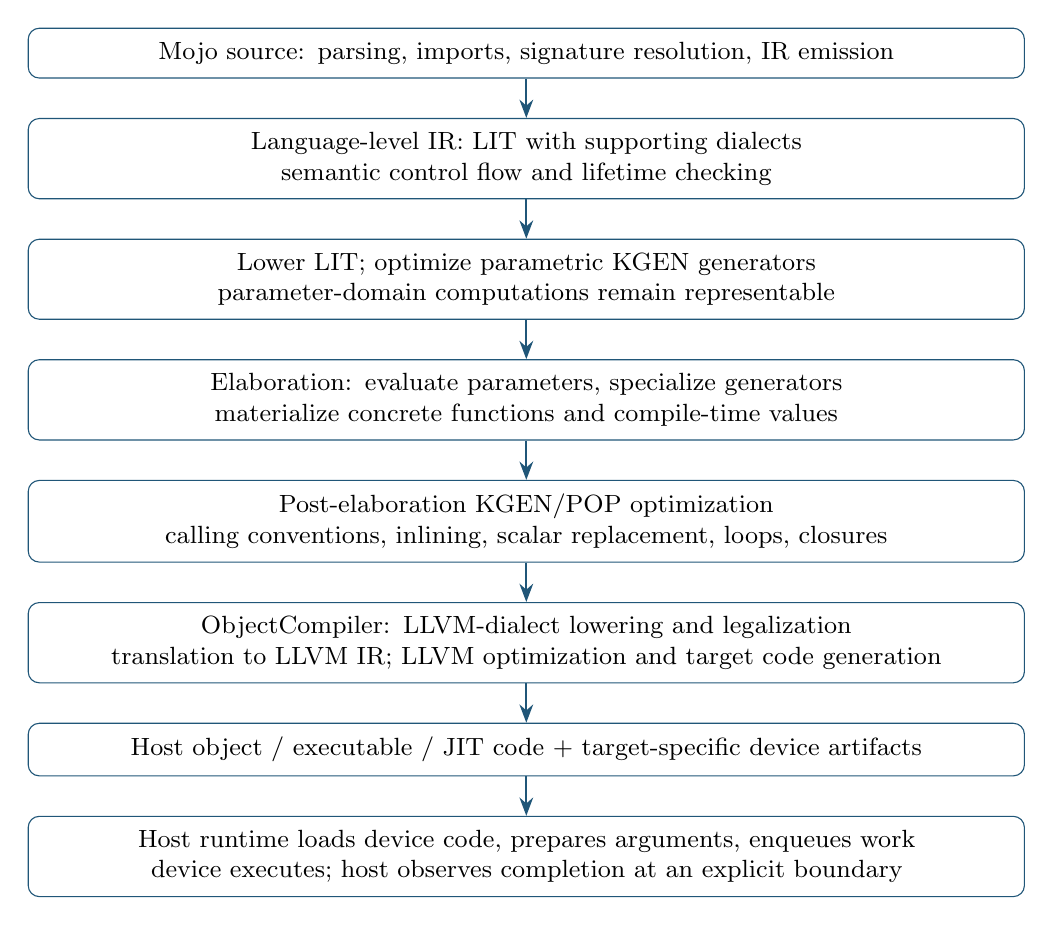
\begin{tikzpicture}[node distance=5mm,box/.style={draw=accent,rounded corners,align=center,text width=123mm,inner sep=5pt,font=\small},arr/.style={-{Stealth},thick,color=accent}]
\node[box] (a) {Mojo source: parsing, imports, signature resolution, IR emission};
\node[box,below=of a] (b) {Language-level IR: LIT with supporting dialects\\semantic control flow and lifetime checking};
\node[box,below=of b] (c) {Lower LIT; optimize parametric KGEN generators\\parameter-domain computations remain representable};
\node[box,below=of c] (d) {Elaboration: evaluate parameters, specialize generators\\materialize concrete functions and compile-time values};
\node[box,below=of d] (e) {Post-elaboration KGEN/POP optimization\\calling conventions, inlining, scalar replacement, loops, closures};
\node[box,below=of e] (f) {ObjectCompiler: LLVM-dialect lowering and legalization\\translation to LLVM IR; LLVM optimization and target code generation};
\node[box,below=of f] (g) {Host object / executable / JIT code + target-specific device artifacts};
\node[box,below=of g] (h) {Host runtime loads device code, prepares arguments, enqueues work\\device executes; host observes completion at an explicit boundary};
\foreach \x/\y in {a/b,b/c,c/d,d/e,e/f,f/g,g/h}\draw[arr] (\x)--(\y);
\end{tikzpicture}
\end{center}
This diagram shows logical milestones. It is not a promise that every command executes every stage, or that the pipeline is a sequence of single-dialect modules. Library generation can stop with parametric code. Compile-time evaluation and offload compilation introduce calls back into compilation infrastructure. Cache hits may reuse earlier work.

The most consequential boundary is \emph{elaboration}: a generator can describe a family of programs, whereas concrete functions can be lowered using ordinary runtime types and flat symbols. A second boundary separates emitted code from loaded, executable code. Producing an artifact does not allocate a GPU buffer or launch a kernel.
\src{Mojo/lib/Compiler/Pipeline/Pipeline.cpp}
\src{Mojo/tools/mojo/Build/mojo-build.cpp}

\chapterpage{Frontend, LIT, and language semantics}
\subsection{What the frontend owns}
The lexer/parser infrastructure recognizes source syntax, imports declarations, resolves signatures, and emits IR. \code{MojoParserContext} offers parsing and tooling entry points, including \code{parseFile}, \code{ensureSignaturesResolved}, and a lighter parsing path for the language server. The source contains AST declaration/type machinery as well as IR emission machinery; describing it as either a conventional full-AST-only frontend or a frontend with no AST at all would hide useful distinctions.

LIT retains language-level abstractions needed to express semantics before lower-level representation choices erase them. Its declared dependencies include KGEN, POP, CO, HLCF, and debug information. An IR dump may therefore mix dialect prefixes even before LIT lowering has completed.

\subsection{Checking before representation loss}
In \code{buildCheckLITPipeline}, \code{createLowerSemanticCF} lowers semantic control-flow operations such as \code{lit.return} to terminators and diagnoses unreachable code. Parameter verification is enabled in non-production builds. \code{createCheckLifetimes} then handles lifetime analysis, destructor insertion, and borrowing checks.

\code{buildLowerLITPipeline} invokes those checks and then \code{createLowerLIT}. This order matters: an ownership or borrowing error should be diagnosed while the representation still explains the source-level relationship. Once an abstraction becomes loads, stores, and raw addresses, the same explanation can be much harder to recover.

\subsection{Ownership and GPU memory are different contracts}
Value semantics, moves, borrowing, and origins describe language-level access and lifetime relationships. Prefer modern \code{Pointer} APIs with appropriate \code{ImmOrigin}/\code{MutOrigin} parameters when writing pointer abstractions. A valid source-level borrow does not by itself prove that an asynchronously launched GPU has finished using the underlying allocation.

Consider a host scope that enqueues a kernel using a device buffer and immediately exits. Correctness also depends on buffer retention, deferred destruction, and the runtime's completion contract. Never infer asynchronous lifetime safety solely from a short lexical scope. Read the concrete buffer/queue API and ensure storage remains valid until the device's last use completes.

\textbf{Inspection exercise.} Find the lifetime pass before \code{createLowerLIT}. Then inspect an existing lifetime regression test and identify which source relationship the diagnostic preserves. Distinguish the test runner named lit from the LIT operations involved in the test.
\src{Mojo/include/Mojo/MojoTooling/ParserDriver.h}
\src{Mojo/lib/Compiler/Pipeline/Pipeline.cpp}
\src{Mojo/include/Mojo/MojoParser/ASTDecl.h}

\chapterpage{KGEN and its supporting dialects}
KGEN supplies top-level and support operations for the kernel generation framework. The compiler uses it for host functions too: the word ``kernel'' does not restrict every KGEN function to GPU execution.

\begin{tabularx}{\linewidth}{@{}p{22mm}X@{}}
\toprule
Dialect & Role in this implementation\\\midrule
\code{lit} & Language-level constructs lowered to KGEN after semantic checking.\\
\code{kgen} & Generators, concrete functions, parameterization, and compilation structure.\\
\code{pop} & Parametric operations layered over the LLVM dialect; later legalized and lowered.\\
\code{hlcf} & Scoped, high-level control flow across nested operations and regions.\\
\code{co} & Parametric coroutine operations for async functions with suspension points.\\
LLVM dialect & MLIR operations representing LLVM-level types and operations before translation to native LLVM IR.\\\bottomrule
\end{tabularx}

These are collaborating representations. In particular, avoid teaching \code{LIT -> HLCF -> POP -> KGEN} as a fixed chronological pipeline. HLCF and POP operations can occur within the same larger compilation unit. Passes lower selected abstractions as their prerequisites become available.

\subsection{Parameters describe programs}
A compile-time parameter can determine a type, SIMD width, selected implementation, or emitted control flow. An ordinary runtime argument supplies data to an already-selected implementation. Both may eventually appear as constants in optimized code, but they start with different semantic contracts.

For example, specializing a function on \code{width=8} can make an eight-lane type legal before runtime optimization begins. Passing the integer 8 as an ordinary argument does not automatically make it available where a compile-time type parameter is required. Later constant propagation may simplify runtime operations, but it does not retroactively make an invalid source program well-typed.

\subsection{Why retain parametric IR?}
Keeping reusable generators supports libraries that can be specialized by a downstream consumer. It also lets optimizations run before duplication across many specializations. However, pre-elaboration inlining can enlarge the interpreter's work and reduce cache granularity. The inspected library pipeline limits parametric inlining to \code{always_inline_no_debug} functions, illustrating a compile-time versus generated-code tradeoff.
\src{Mojo/include/Mojo/KGENDialect/KGENDialect.td}
\src{Mojo/include/Mojo/POPDialect/POPDialect.td}
\src{Mojo/include/Mojo/HLCFDialect/HLCFDialect.td}
\src{Mojo/include/Mojo/CODialect/CODialect.td}

\chapterpage{Elaboration and compile-time execution}
\subsection{Three related operations}
\textbf{Specialization} fixes parameters of a reusable definition. \textbf{Compile-time evaluation} computes values during compilation. \textbf{Materialization} gives a compile-time result the runtime representation needed by residual code. Elaboration coordinates these concerns; it is broader than replacing one symbolic integer with a constant.

\lstinputlisting{examples/specialization.mojo}
This CPU example should print \code{11}. The parameter \code{bias} and the local \code{comptime} result are compile-time values; \code{x} is a runtime argument in the function definition. The call in \code{main} has a constant operand, so optimization may fold even more of the program than elaboration alone requires.

The following is \textbf{schematic IR reasoning}, not parseable MLIR or a promised compiler dump:
\begin{lstlisting}
Generator add_bias[bias](x): return x + bias
Elaborate add_bias[3]  -> concrete add_bias_3(x): return x + 3
Evaluate add_bias[3](4) at compile time -> 7
Residual main         -> print(add_bias_3(8))
Further optimization  -> may fold the remaining call to 11
\end{lstlisting}
The residual call receives \code{folded + 1}, namely 8, and produces 11. An optimized dump may contain only the final value and printing machinery, so disappearance of the specialized function is an expected possibility.

\subsection{The implementation sequence}
\code{buildElaborateModulePipeline} eliminates dead symbols, outlines closures, optionally runs CSE, lifts/folds apply operations, and reorders parameter operations. It then invokes \code{createElaborateGenerators} with target information and callbacks for assembly/offload compilation. Options control interpreter choice, diagnostics, maximum depth, and loop-unrolling warnings.

\code{KGENCompiler} exposes \code{runGenerateLibraryPipeline}, \code{runElaborationPipeline}, and \code{runKGENPipeline}. Their scopes differ: the elaboration entry point does not itself include LIT checking and all pre-elaboration preparation. Use the intended entry point for the input's phase.

The header also provides a default specialization executor that JIT-compiles and executes in-process. Consequently, an ahead-of-time application build can still involve execution during compilation. This does not make the final application dependent on replaying every compile-time evaluation at startup.
\src{Mojo/include/Mojo/Compiler/KGENCompiler.h}
\src{Mojo/lib/Compiler/Pipeline/Pipeline.cpp}

\chapterpage{Post-elaboration optimization and invariants}
After elaboration, the compiler can optimize concrete functions without carrying unresolved parameter structure into every backend pass. In the inspected implementation, the post-elaboration pipeline first applies the floating-point policy, verifies elaborated IR, and updates materialized values before the main optimization pipelines.

\subsection{Materialization has a memory consequence}
\code{createUpdateMaterialization} runs before SROA and Mem2Reg. Its source comment explains the hazard: pointers to materialized values may still refer to interpreter storage. If the compiler reasons about the wrong storage, a destination can appear not to escape and be scalarized away. This is a useful example of phase ordering preserving correctness rather than merely improving performance.

\subsection{First and late optimization pipelines}
The first pipeline deduplicates functions, eliminates dead symbols, resolves compiler promises, lowers argument and calling conventions, and infers function attributes. Automatic inlining contains its own function optimization pipeline. Scalar replacement, memory-to-register promotion, canonicalization, loop handling, and conditional constant propagation expose simpler code.

The late pipeline performs additional optimization depending on the optimization level, then lowers loops, closures, and async functions. Dead argument and symbol elimination remove residual overhead. Some simplification passes run even at low optimization levels because downstream representation and language implementation still require them.

\subsection{How to assess an optimization}
For a tiled AI kernel, ask a precise question: did a constant tile width remove a bounds branch, or did inlining expose adjacent loads for vectorization? Compare the earliest IR where the transformation should become legal with a later dump. A change in assembly alone does not identify which pass caused it.

Preserve numerical requirements while experimenting. Reassociation, contraction, and reduced precision are distinct choices. A faster reduction that changes the intended floating-point behavior needs a separately stated accuracy contract and error measurements.

\textbf{Review exercise.} Explain why moving materialization repair after SROA could be wrong. Then identify which transformations are guarded by \code{optimizationLevel >= 1} or \code{>= 2}. Expected result: a table separating semantic/representation requirements from optional optimization, based on the actual source guards.
\src{Mojo/lib/Compiler/Pipeline/Pipeline.cpp}

\chapterpage{ObjectCompiler, LLVM lowering, and artifacts}
\code{M::KGEN::ObjectCompiler} is an internal C++ compilation component. Its header defines its purpose as lowering concrete KGEN functions to LLVM and then to objects. It is not a Mojo user-facing object that allocates accelerator memory.

\begin{tabularx}{\linewidth}{@{}p{63mm}X@{}}
\toprule
Entry point & Responsibility\\\midrule
\code{create} & Resolve a registered backend from compilation options and construct the compiler.\\
\code{lowerAllFuncsToLLVM} & Produce an \code{llvm::Module} from the input module.\\
\code{lowerAllFuncsToLLVMAndOptimize} & Lower and run LLVM optimization.\\
\code{emitArchive} & Emit an object archive, with an optional cache-key hash output.\\
\code{emitLLVMIR}, \code{emitAssembly} & Emit inspectable code for exported-symbol reachability.\\
\code{emitSharedObject} & Emit a shared object for the relevant target/linking path.\\
\code{emitOffloadKernels} & Produce requested emission kinds for offloaded kernels.\\\bottomrule
\end{tabularx}

\subsection{LLVM dialect is not LLVM IR}
The lowering pipeline invokes KGEN-to-LLVM conversion, runtime closure lowering, POP legalization, global/function POP lowering, control-flow lowering, cast reconciliation, and suspension-point lowering. Canonicalization and CSE follow. A target-specific late lowering hook runs before final debug-info lowering.

At this point operations still belong to an MLIR module. Translation subsequently produces native LLVM IR, represented by \code{llvm::Module}. LLVM optimization and target code generation then produce lower-level artifacts. A file containing LLVM-dialect MLIR is not interchangeable with textual LLVM IR accepted by LLVM tools.

\subsection{The build driver makes the handoff}
\code{mojo-build.cpp} constructs \code{KGENCompiler} and \code{ObjectCompiler}, runs the KGEN pipeline, and then chooses the requested emission path. It also configures offload output prefixes for relevant emission kinds before the KGEN pipeline runs. Thus a heterogeneous build can emit host output and associated device output.

A CPU object, LLVM bitcode, PTX, a device binary, and a shared library satisfy different loading contracts. Assembly text is not universally a directly executable binary. Inspect the target backend's supported emission kinds instead of assuming every output format works for every accelerator.
\src{Mojo/include/Mojo/Compiler/ObjectCompiler.h}
\src{Mojo/lib/Compiler/ObjectCompiler/KGENToLLVMPipeline.cpp}
\src{Mojo/tools/mojo/Build/mojo-build.cpp}

\chapterpage{Targets, execution engines, and compilation caches}
\subsection{Target selection is a semantic input}
A target triple describes the platform and binary conventions. CPU and feature selection constrain usable instructions and layouts. Accelerator selection constrains device code. Host and device compilation can therefore require different targets within the same application.

\code{ObjectCompiler::create} resolves the backend from the requested target and reports unsupported targets. \code{TargetBackend} is the code-generation abstraction to inspect when extending target support. A backend implementation alone does not supply the device memory, loading, synchronization, or launch APIs required to execute on new hardware.

\subsection{AOT and JIT share infrastructure}
Object generation and execution are separate services. \code{ExecutionEngine} uses LLVM ORC infrastructure for executable code and symbol handling. Its options include libraries, debug/profiling integration, and a cross-compiling mode that forgoes JIT setup. \code{initializeExecutionEngine} wires together compilation options, caches, target setup, and the engine.

This gives three different events that people may call ``compilation'': compiling the application, evaluating compiler-time functions, and preparing a device function for execution. Measure and name them separately. \code{DeviceContext.compile_function} does not prove that the runtime reparses Mojo source on every call.

\subsection{Caching changes performance observations}
\code{ObjectCompiler} owns a transform cache; the elaboration interface also supports cached transforms. Object emission has paths for parallel LLVM code generation and later machine-code linking. These details explain why wall-clock compilation time cannot be inferred from the sum of pass times alone.

For a compile-time regression, record compiler revision, target, optimization flags, cache state, source changes, and output kind. Report first-build and repeated-build measurements independently. Do not assume a cache key is merely a source filename: target and compilation configuration affect correctness. Consult the actual key construction before making claims about invalidation.

For a runtime benchmark, distinguish device-code preparation and module loading from repeated launches. A fast second iteration can reflect cache warming, allocation reuse, or device initialization rather than an improved generated kernel.
\src{Mojo/include/Mojo/Compiler/Target/TargetBackend.h}
\src{Mojo/include/Mojo/ExecutionEngine/ExecutionEngine.h}
\src{Mojo/include/Mojo/Compiler/KGENCompiler.h}
\src{Mojo/include/Mojo/Compiler/ObjectCompiler.h}

\chapterpage{Driver layers and the runtime boundary}
\subsection{The command driver}
The \code{mojo} tool dispatches subcommands such as build and run. Build processing selects options, input handling, compilation, output, and linking behavior. This is where a wrong output format or target configuration should be investigated before assuming a device runtime failure.

\subsection{MAX Driver APIs}
The Python package \code{max.driver} provides device-oriented interfaces. In this snapshot, \code{driver.py} imports \code{CPU}, \code{Accelerator}, \code{Device}, and \code{DeviceQueue} from \code{max._core.driver}. Buffer behavior is implemented/exposed through accompanying modules. This layer supports Python orchestration; it is not a mandatory extra Python call in every standalone Mojo GPU program.

\subsection{Mojo to AsyncRT to the device implementation}
The Mojo \code{DeviceContext} wrapper contains external calls such as:
\begin{lstlisting}
AsyncRT_DeviceContext_create
AsyncRT_DeviceContext_createBuffer_async
AsyncRT_DeviceContext_loadFunction
AsyncRT_DeviceContext_enqueueFunctionDirect
AsyncRT_DeviceContext_retain
AsyncRT_DeviceContext_release
\end{lstlisting}
These names are source navigation anchors, not a supported application ABI to reproduce manually. They expose the boundary between the Mojo host API and runtime services. The inspected wrapper documents \code{enqueue} as forwarding directly to the default-stream enqueue function.

Below that boundary, the runtime must arrange platform-specific loading and execution through the selected device API. Exact vendor implementation details must be checked in the corresponding runtime implementation; the wrapper alone does not establish every CUDA, HIP, or Metal call made underneath it.

\subsection{Errors belong to different timelines}
A parser diagnostic occurs before object generation. A linker error concerns missing/incompatible symbols or libraries. Device initialization can fail after host compilation succeeds. Launch configuration errors may be detected during enqueue; execution failures may surface at a later synchronization point.

For debugging, record the first failing operation and the next observed completion boundary. If adding synchronization after a launch localizes an error, that is diagnostic evidence, not a reason to keep every launch synchronized in a throughput-sensitive production loop.
\src{Mojo/tools/mojo/mojo.cpp}
\src{max/python/max/driver/driver.py}
\src{max/python/max/driver/buffer.py}
\src{max/mojo/max/gpu/host/device_context.mojo}

\chapterpage{DeviceContext, buffers, streams, and DeviceFunction}
\code{DeviceContext} is a host-side accelerator interface centered on a stream. This snapshot also exposes richer stream management. Reason about each operation's stream; a context is not an implicit global barrier.

The API supports allocation, transfers, function preparation, enqueue, and synchronization. Its context-manager interface and retain/release calls manage runtime resources.

\subsection{The kernel handle}
\code{DeviceFunction} represents a compiled device function and manages compilation information, loading, and resources. Its parameters include the function, declared argument types, target, and compile/link options. It contains \code{CompiledFunctionInfo}. A separate \code{DeviceExternalFunction} represents externally supplied device code.

\code{compile_function} prepares a reusable function handle. \code{enqueue_function} offers convenience paths that prepare and launch a function, plus overloads for existing/external functions. Overload details and output-parameter conventions evolve; inspect the installed SDK before copying an older example.

\subsection{Minimal GPU lifecycle}
\lstinputlisting[basicstyle=\ttfamily\footnotesize,firstline=2]{examples/gpu_hello.mojo}
The expected result is four lines whose thread indices cover 0 through 3, followed by \code{complete}. Device print ordering is unspecified. This is a launch/lifecycle smoke test, not a performance benchmark. It requires the matching MAX Mojo package and a supported accelerator/runtime installation.

\subsection{Ordering and lifetime}
Operations on an ordered stream can rely on that stream's sequencing contract. Independent streams need explicit dependencies when one consumes another's results. A host dereference of device memory is not made valid by having a pointer-shaped value. Use the appropriate transfer or mapping operation and wait for completion before consuming results on the host.

Keep buffers and function resources valid for outstanding work. Ownership and completion are separate contracts. For overlap, use multiple buffers and events, then verify dependencies before measuring throughput.
\src{max/mojo/max/gpu/host/device_context.mojo}

\chapterpage{End-to-end AI kernel: vector addition}
Consider \(C_i=A_i+B_i\) for \(0\le i<N\), implemented as one GPU thread per element. The following is \textbf{pseudocode}; it intentionally abstracts the SDK's current buffer constructors and pointer signatures:
\begin{lstlisting}
compile-time: choose Float32 element type and kernel target
kernel(A, B, C, N):
    i = block_idx.x * block_dim.x + thread_idx.x
    if i < N:
        C[i] = A[i] + B[i]

host:
    create context and allocate A, B, C on its device
    enqueue copies of initialized host A and B
    prepare kernel; enqueue with block_dim = Bsize
    grid_dim = ceil_div(N, Bsize)
    enqueue copy of C back to host
    wait for the stream's work to complete
    compare every C[i] against the reference A[i] + B[i]
\end{lstlisting}

\subsection{Follow the responsibilities}
The frontend checks the function and pointer operations. LIT lowering discharges language abstractions. Specialization fixes element types and target-dependent choices. KGEN optimization simplifies the concrete body. Object compilation lowers address arithmetic, loads, addition, stores, and device indexing into target code. Runtime preparation loads the kernel and packs its arguments; enqueue submits its launch geometry.

\(N\) can remain a runtime argument. The compiler need not generate a new specialization for every input length. A compile-time block/tile choice may enable a more specialized implementation, but indiscriminate specialization across shapes, types, and targets can multiply compilation cost and code size.

\subsection{Correctness and performance experiments}
Test \(N=1\), \(N=Bsize-1\), \(N=Bsize\), and \(N=Bsize+1\), plus a larger nonmultiple. Decide explicitly how the host handles \(N=0\); a zero-sized launch is not a portable assumption. Check bounds protection and output completeness before timing.

For Float32 addition, the idealized traffic is two 4-byte reads and one 4-byte write per element, or \(12N\) bytes. Effective bandwidth is \(12N/t\), where \(t\) measures device kernel time with clearly stated cache assumptions. This estimate omits transfers and runtime overhead. End-to-end latency must include those separately.

A host timer around an asynchronous enqueue measures submission, not completion. Warm up code loading and allocation, time completed work, and report distributions. Use events or a deliberate completion boundary. Then inspect coalescing, launch size, occupancy, and register pressure; increasing block size does not guarantee higher throughput.

\chapterpage{Hands-on inspection and debugging labs}
\subsection{Lab 1: CPU specialization and emitted code}
Use a matching nightly toolchain; these commands run from this guide's folder:
\begin{lstlisting}
mojo --version
mojo build --help
mojo run examples/specialization.mojo
mkdir -p build
mojo build examples/specialization.mojo --emit llvm -o build/specialization.ll
mojo build examples/specialization.mojo --emit asm -o build/specialization.s
\end{lstlisting}
Expected output from the run is \code{11}. Inspect whether the call remains or has been folded. LLVM emission is not necessarily fully LLVM-optimized IR; the inspected build path calls \code{lowerAllFuncsToLLVM} for this output. Compare with assembly and consult output-kind help before naming a dump ``optimized''.

\subsection{Lab 2: locate internal phase boundaries}
From the Modular source root:
\begin{lstlisting}
rg -n 'buildCheckLITPipeline|createLowerLIT|createElaborateGenerators' Mojo/lib/Compiler/Pipeline/Pipeline.cpp
rg -n 'createUpdateMaterialization|buildFirstOptPipeline|buildLateOptPipeline' Mojo/lib/Compiler/Pipeline/Pipeline.cpp
rg -n 'runKGENPipeline|ObjectCompiler::create' Mojo/tools/mojo/Build/mojo-build.cpp
rg -n 'createLowerKGENToLLVM|createLowerPOPToLLVM' Mojo/lib/Compiler/ObjectCompiler/KGENToLLVMPipeline.cpp
\end{lstlisting}
Record each stage's input contract and output invariant. For pass-level IR, inspect \code{PassManagerConfigOptions} and compiler/test tool help in the matching checkout. Internal MLIR printing flags are not guaranteed public \code{mojo build} options; do not assume that a generic MLIR flag or an invented \code{--emit lit} mode is supported.

\subsection{Lab 3: device preparation versus execution}
Run \code{mojo run examples/gpu_hello.mojo} on a supported GPU installation. Then inspect the \code{dump_asm} and \code{dump_llvm} parameters of the current \code{compile_function}/\code{enqueue_function} overload. Device dumps and host assembly answer different questions. Compare first invocation with repeated launches using a non-printing kernel before drawing performance conclusions.

\textbf{Validation status.} The guide's LaTeX/PDF build is checked separately from these labs. No matching Mojo SDK was available on PATH. A cached March 2026 compiler reported version 0.26.3.0.dev2026031705 but crashed when attempting the CPU example. Neither example has validated execution. The examples follow the inspected source syntax; the GPU example follows the wrapper's documented usage.

\chapterpage{Source reading map and review questions}
Use the source anchors below in order. Paths are relative to the baseline checkout; a public distribution may expose a different subset of internals.

\begin{enumerate}
\item \nolinkurl{Mojo/tools/mojo/Build/mojo-build.cpp}: command processing and handoff between the KGEN and object compilers.
\item \nolinkurl{Mojo/include/Mojo/MojoTooling/ParserDriver.h}: frontend/tooling context and parsing APIs.
\item \nolinkurl{Mojo/include/Mojo/LITDialect/LITDialect.td}: language-level IR contract and dependencies.
\item \nolinkurl{Mojo/lib/Compiler/Pipeline/Pipeline.cpp}: LIT checks, library generation, elaboration, and post-elaboration optimization.
\item \nolinkurl{Mojo/include/Mojo/Compiler/KGENCompiler.h}: pipeline entry-point contracts.
\item \nolinkurl{Mojo/include/Mojo/Compiler/ObjectCompiler.h}: object generation and cache interfaces.
\item \nolinkurl{Mojo/lib/Compiler/ObjectCompiler/KGENToLLVMPipeline.cpp}: late MLIR legalization/lowering.
\item \nolinkurl{Mojo/include/Mojo/ExecutionEngine/ExecutionEngine.h}: compiled functions and ORC execution infrastructure.
\item \nolinkurl{max/mojo/max/gpu/host/device_context.mojo}: buffers, function handles, streams, launch packing, and AsyncRT external calls.
\item \nolinkurl{max/python/max/driver/driver.py}: Python device API boundary.
\end{enumerate}

\subsection{Review questions with expected reasoning}
\begin{enumerate}
\item \textbf{Why can KGEN appear before and after elaboration?} The dialect supports parametric generators and concrete compilation structure; its presence alone does not identify the phase.
\item \textbf{Does an AOT build rule out JIT activity?} No. Compile-time evaluation may use a JIT executor even when the final product is an executable.
\item \textbf{Why can compilation succeed but launch fail?} Artifact generation and runtime device/ABI/resource validity are separate contracts.
\item \textbf{Why might more inlining slow compilation?} Parametric expansion increases elaboration work and can reduce reuse; later inlining may recover runtime performance with less early duplication.
\item \textbf{Does ownership prove GPU completion?} No. Storage/access validity and asynchronous dependencies must both be satisfied.
\end{enumerate}

\chapterpage{Public references and further experiments}
These official references complement the snapshot-specific source anchors. Public documentation describes supported interfaces; internal implementation details in this guide come from the inspected checkout.

\begin{enumerate}
\item \href{https://mojolang.org/docs/tools/compilation/}{Mojo: Compilation targets}. Target selection and emitted artifact options. The public command examples in the labs use its LLVM/assembly emission interface.
\item \href{https://max.modular.com/stable/api/mojo/max/gpu/host/device_context/DeviceContext/}{MAX: DeviceContext API}. Public host-side accelerator interface. Compare its versioned signatures with the local nightly source before adapting examples.
\item \href{https://mojolang.org/docs/}{Mojo documentation}. Entry point for the language manual and release-specific syntax.
\end{enumerate}

\subsection{Suggested advanced projects}
\textbf{Specialization budget.} Implement a family of elementwise kernels with a small fixed set of tile widths, then compare against unrestricted shape specialization. Record compilation time, generated code size, warm execution time, and numerical correctness. Explain which dimensions truly need to be parameters.

\textbf{Phase-local regression.} Choose a small existing compiler regression test. Identify the earliest pass where the property is expressible, inspect nearby tests and BUILD targets, and add one minimal case. From the Modular root, discover targets with \code{./bazelw query}; run the specific test using \code{./bazelw test //path:target}. Do not use a full repository test run as the first experiment.

\textbf{Transfer/compute overlap.} Replace a serialized copy--kernel--copy loop with double buffering and explicit dependencies. Validate all outputs, then compare completed end-to-end throughput and device utilization. Explain which stream waits on which event and why no allocation is reclaimed too early.

\textbf{Backend exploration.} Trace a supported \code{TargetBackend} from registration to artifact emission, then identify what a hypothetical new accelerator would need beyond code generation: runtime discovery, memory, module loading, argument ABI, launches, events, diagnostics, and tests. Separate source portability from binary portability.

\subsection{Maintenance checklist}
On a new compiler revision, update the baseline commit, re-check pass order and entry-point contracts, run both examples with the matching SDK, and rebuild this PDF. Keep code snippets and example files synchronized through \code{lstinputlisting}. Recheck public links and document actual validation outcomes rather than preserving old success claims.
\end{document}
